

\section{Introduction}

\begin{frame}{Introduction}{Analysis goal}
Measurement of the triple gauge couplings in the WW final state
\begin{itemize}
%
  \item CLIC is a gauge boson factory
  \item important for EFT\footnote{Effective Field Theory} analyses \href{https://link.springer.com/content/pdf/10.1007/JHEP05(2017)096.pdf}{JHEP 05, 096 (2017)}
  \begin{itemize}
  %
    \item scale of new physics is large and EFT serves as low energy description
  %
  \end{itemize}
  \item chose \qqln\ final state:
%
\end{itemize}

\begin{figure}
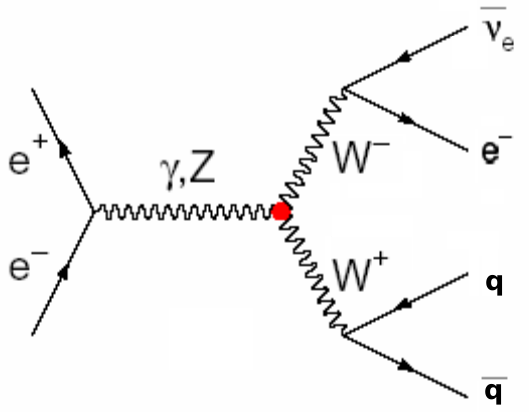
\includegraphics[width=0.25\textwidth]{triple_gauge_s_chan.png} \hspace{1em}
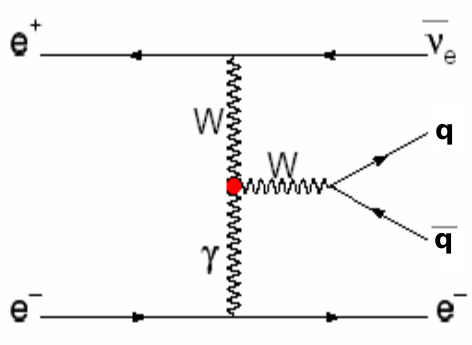
\includegraphics[width=0.25\textwidth]{triple_gauge_t_chan.png} \hspace{1em}
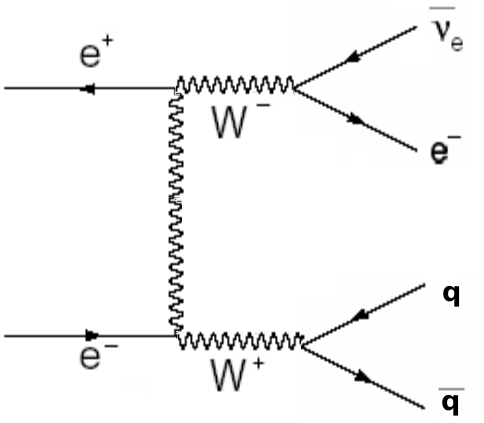
\includegraphics[width=0.25\textwidth]{triple_gauge_bkg.png}
\caption{
  The two main processes in \epm\ collisions for triple gauge couplings (marked in red) and the main background process.
}
\end{figure}

\end{frame}

